%@ chapter=1
%@ exercise=11
%@ author=Fabian

\begin{enumerate}
\item In fact, $M(f)$ is a function with domain $A^*$ and codomain $B^*$ for $f : A → B$ and it remains to show that it is a homomorphism and that $M$ respects arrow composition as well as identity.

	Firstly, the empty word $ε_A$ in $A^*$ is mapped to the empty product $M(f)(ε_A) = ε_B$, which is the empty word in $B^*$. Secondly, the product of two words $w_1 = a_1 … a_n, w_2 = b_1 … b_m$ is mapped to $f(a_1) … f(a_n)f(b_1) … f(b_m)$ by definition, which by associativity is the same as $M(f)(w_1)M(f)(w_2)$. Thus, $M(f)$ is a homomorphism and an arrow between $M(A)$ and $M(B)$ in category $\cat{Mon}$.

	$M$ distributes over arrow composition by the following succession of equalities.

	\begin{align*}
	M(f ∘ g)(a_1 … a_n) & = (f ∘ g)(a_1) … (f ∘ g)(a_n) \\
	& = f(g(a_1)) … f(g(a_n) \\
	& = M(f)(g(a_1) … g(a_n)) \\
	& = M(f)(M(g)(a_1 … a_n)) \\
	& = (M(f) ∘ M(g))(a_1 … a_n)
	\end{align*}

	Lastly, $M$ maps the identity function on a set to the identity homomorphism between (free) monoids.

	Therefore, $M$ is a functor from $\cat{Set}$ to $\cat{Mon}$.

\item We want to define $M(f)$ given $f : A → B$. In $\cat{Set}$ we obtain the following diagram, which we will apply the UMP of the free monoid $A^*$ to.

	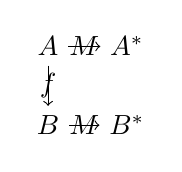
\begin{tikzpicture}
	  \node (A) {$A$};
	  \node (A*) [right of=A] {$A^*$};
	  \node (B) [below of=A] {$B$};
	  \node (B*) [right of=B] {$B^*$};
	  \draw[->] (A) to node {$M$} (A*);
	  \draw[->] (B) to node {$M$} (B*);
	  \draw[->] (A) to node {$f$} (B);
	\end{tikzpicture}

	Considering the composition arrow $M ∘ f$ there exists a unique monoid homomorphism $u : A^* → B^*$ so that following diagram in $\cat{Set}$ commutes.

	\begin{tikzpicture}
	  \node (A) {$A$};
	  \node (A*) [right of=A] {$A^*$};
	  \node (B*) [below of=A*] {$B^*$};
	  \draw[->] (A) to node {$M$} (A*);
	  \draw[->] (A) to node {$M ∘ f$} (B*);
	  \draw[->, dashed] (A*) to node {$u$} (B*);
	\end{tikzpicture}

	Now, let $M(f)$ the arrow corresponding to $u$ in $\cat{Mon}$ and prove that this definition of $M$ respects arrow composition as well as identity arrows. Therefore, consider the following diagram in $\cat{Set}$.

	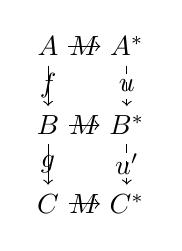
\begin{tikzpicture}
	  \node (A) {$A$};
	  \node (A*) [right of=A] {$A^*$};
	  \node (B) [below of=A] {$B$};
	  \node (B*) [right of=B] {$B^*$};
	  \node (C) [below of=B] {$C$};
	  \node (C*) [right of=C] {$C^*$};
	  \draw[->] (A) to node {$M$} (A*);
	  \draw[->] (B) to node {$M$} (B*);
	  \draw[->] (C) to node {$M$} (C*);
	  \draw[->] (A) to node {$f$} (B);
	  \draw[->] (B) to node {$g$} (C);
	  \draw[->, dashed] (A*) to node {$u$} (B*);
	  \draw[->, dashed] (B*) to node {$u'$} (C*);
	\end{tikzpicture}

	Since $u' ∘ u : A^* → C^*$ is a monoid homomorphism and $M(g ∘ f)$ is the unique homomorphism from $A^*$ to $C^*$ we have $M(g ∘ f) = u' ∘ u = M(g) ∘ M(f)$. Furthermore, $id_{A^*}$ is obviously a monoid endomorphism so that $M(id_A) = id_{A^*}$ and, hence, $M$ is a functor.

\item The second approach does not repeat the existence proof of the free monoid but exploits its essential features (existence, uniqueness of the monoid homomorphism) which are captured in the UMP. The first approach gives us (the only possible) way to compute a monoid structure preserving mapping on (the free) monoid that coincides with a arbitrarily chosen mapping on some set.
\end{enumerate}
